\begin{figure}[!tbh]
  \resizebox{.45\linewidth}{!}{
    \centering  
    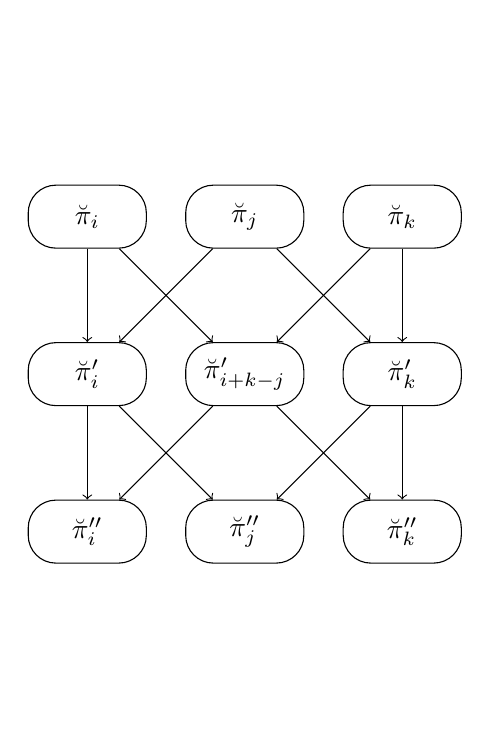
\begin{tikzpicture}
      \tikzstyle{STY1} = [draw, rectangle, minimum height=.8cm, minimum width=1.5cm, rounded corners=10pt]
      \tikzstyle{STY2} = [->]

      %%%%% VERTEX

      \node[draw=none, fill=none, rectangle, minimum height=.8cm, minimum width=1.5cm, rounded corners=10pt](v0) at ({(2*2 - 2)}, 2.0) {};

      \node[STY1](v1) at ({(2*1 - 2)}, 0.0) {$\breve\pi_i$};
      \node[STY1](v2) at ({(2*2 - 2)}, 0.0) {$\breve\pi_j$};
      \node[STY1](v3) at ({(2*3 - 2)}, 0.0) {$\breve\pi_k$};

      \node[STY1](v4) at ({(2*1 - 2)}, -2.0) {$\breve\pi^{\prime}_i$};
      \node[STY1](v5) at ({(2*2 - 2)}, -2.0) {$\breve\pi^{\prime}_{i+k-j}$};
      \node[STY1](v6) at ({(2*3 - 2)}, -2.0) {$\breve\pi^{\prime}_k$};


      \node[STY1](v7) at ({(2*1 - 2)}, -4.0) {$\breve\pi^{\prime\prime}_i$};
      \node[STY1](v8) at ({(2*2 - 2)}, -4.0) {$\breve\pi^{\prime\prime}_j$};
      \node[STY1](v9) at ({(2*3 - 2)}, -4.0) {$\breve\pi^{\prime\prime}_k$};

      \node[draw=none, fill=none, rectangle, minimum height=.8cm, minimum width=1.5cm, rounded corners=10pt](v10) at ({(2*2 - 2)}, -6.0) {};

      %%%%% EDGES

      \draw[STY2]  (v1) edge (v4);
      \draw[STY2]  (v1) edge (v5);
      \draw[STY2]  (v2) edge (v4);
      \draw[STY2]  (v2) edge (v6);
      \draw[STY2]  (v3) edge (v5);
      \draw[STY2]  (v3) edge (v6);

      \draw[STY2]  (v4) edge (v7);
      \draw[STY2]  (v4) edge (v8);
      \draw[STY2]  (v5) edge (v7);
      \draw[STY2]  (v5) edge (v9);
      \draw[STY2]  (v6) edge (v8);
      \draw[STY2]  (v6) edge (v9);
      %     \node[draw=none,fill=none, minimum height=1cm, minimum width=1cm] at (0.0, 2.0) {a)};
    \end{tikzpicture}
  }
  \hfill
  \resizebox{.45\linewidth}{!}{
    \centering
    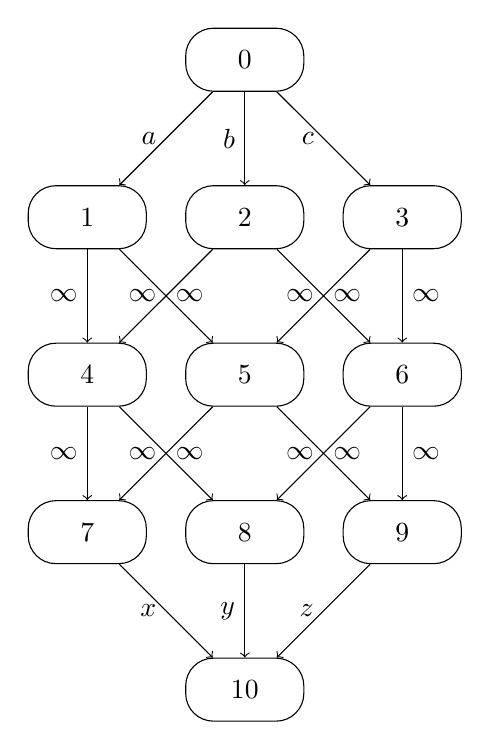
\begin{tikzpicture}
      \tikzstyle{STY1} = [draw, rectangle, minimum height=.8cm, minimum width=1.5cm, rounded corners=10pt]
      \tikzstyle{STY2} = [->]

      %%%%% VERTEX

      \node[STY1](v0) at ({(2*2 - 2)}, 2.0) {0};

      \node[STY1](v1) at ({(2*1 - 2)}, 0.0) {1};
      \node[STY1](v2) at ({(2*2 - 2)}, 0.0) {2};
      \node[STY1](v3) at ({(2*3 - 2)}, 0.0) {3};

      \node[STY1](v4) at ({(2*1 - 2)}, -2.0) {4};
      \node[STY1](v5) at ({(2*2 - 2)}, -2.0) {5};
      \node[STY1](v6) at ({(2*3 - 2)}, -2.0) {6};


      \node[STY1](v7) at ({(2*1 - 2)}, -4.0) {7};
      \node[STY1](v8) at ({(2*2 - 2)}, -4.0) {8};
      \node[STY1](v9) at ({(2*3 - 2)}, -4.0) {9};

      \node[STY1](v10) at ({(2*2 - 2)}, -6.0) {10};

      %%%%% EDGES
      \draw[STY2]  (v0) edge node[anchor=center, left, midway] {$a$} (v1);
      \draw[STY2]  (v0) edge node[anchor=center, left, midway] {$b$} (v2);
      \draw[STY2]  (v0) edge node[anchor=center, left, midway] {$c$} (v3);

      \draw[STY2]  (v1) edge node[anchor=center, left, midway] {$\infty$} (v4);
      \draw[STY2]  (v1) edge node[anchor=center, left, midway] {$\infty$} (v5);
      \draw[STY2]  (v2) edge node[anchor=center, right, midway] {$\infty$} (v4);
      \draw[STY2]  (v2) edge node[anchor=center, left, midway] {$\infty$} (v6);
      \draw[STY2]  (v3) edge node[anchor=center, right, midway] {$\infty$} (v5);
      \draw[STY2]  (v3) edge node[anchor=center, right, midway] {$\infty$} (v6);

      \draw[STY2]  (v4) edge node[anchor=center, left, midway] {$\infty$} (v7);
      \draw[STY2]  (v4) edge node[anchor=center, left, midway] {$\infty$} (v8);
      \draw[STY2]  (v5) edge node[anchor=center, right, midway] {$\infty$} (v7);
      \draw[STY2]  (v5) edge node[anchor=center, left, midway] {$\infty$} (v9);
      \draw[STY2]  (v6) edge node[anchor=center, right, midway] {$\infty$} (v8);
      \draw[STY2]  (v6) edge node[anchor=center, right, midway] {$\infty$} (v9);

      \draw[STY2]  (v7) edge node[anchor=center, left, midway] {$x$} (v10);
      \draw[STY2]  (v8) edge node[anchor=center, left, midway] {$y$} (v10);
      \draw[STY2]  (v9) edge node[anchor=center, left, midway] {$z$} (v10);

      %     \node[draw=none,fill=none, minimum height=1cm, minimum width=1cm] at (0.0, 2.0) {b)};
    \end{tikzpicture}
  }
  \caption[Exemplo de fluxo de nucleotídeos entre as regiões intergênicas.]{No lado esquerdo, uma representação do fluxo de nucleotídeos entre as regiões intergênicas. No lado direito, a instância $I_{MF}$ do problema de fluxo máximo com os vértices de origem (0) e destino (10).}
  \label{figure:XUQWDNIW}
\end{figure}